\part{Conclusion}

\section{Concluding remarks}
We have reviewed how rasterization and ray tracing techniques can be combined to make steps towards photo-realistic, real-time rendering. We identified that the deferred rendering pipeline was a good choice for the rasterization stages, since it easily allows the rasterized g-buffer data to be stored in view space. This is the same space that is output from a raytracer, and makes it simpler to mix the results from the two different rendering techniques.

\begin{figure}[H]
	\centering
	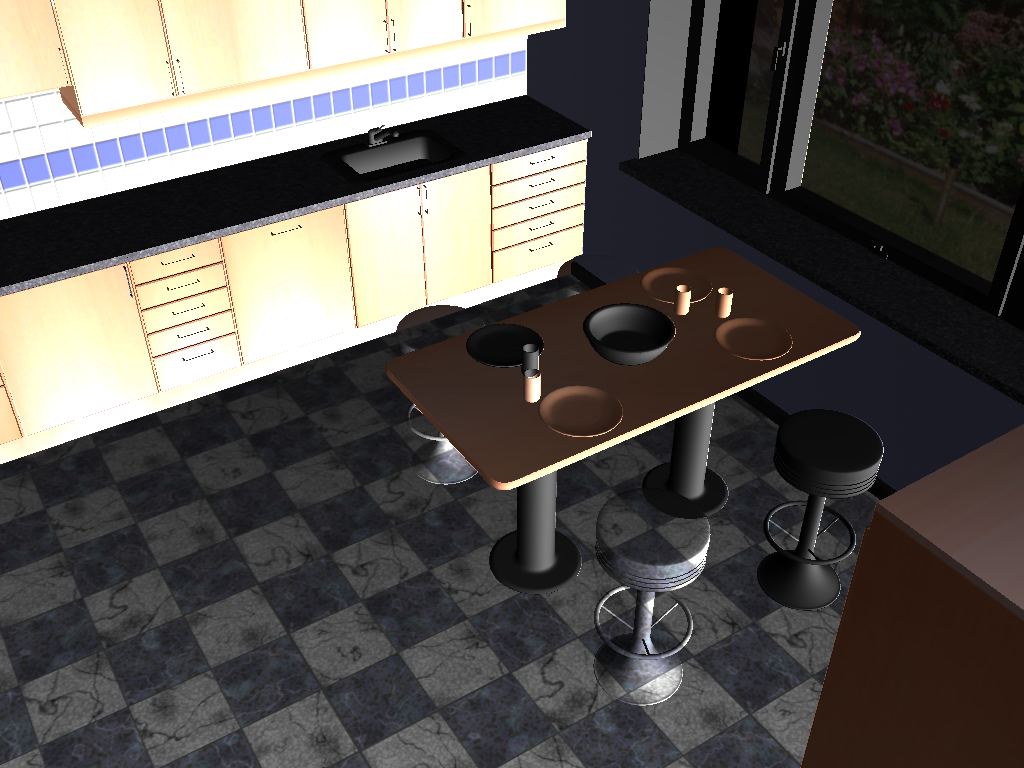
\includegraphics[width=1.00\textwidth]{Media/hybrid.png}
	\caption{Geometry rasterized, normals raytraced. Three of the chairs, and some of the dishes, were only raytraced.}
	\label{fig:hybrid_image01}
\end{figure}

The OptiX raytracer API was a good choice for the dissertation work, since it was a complete raytracer implemented on top of Cuda, with accelerated structure support and it's interopability based on Cuda's strong foundation.

In our Hybridity chapters, we identified several rendering problems where the raytracer would be stronger than a rasterizer. Order independent transparency, aliasing-free shadows, reflections and refractions, analytical geometry and volumetric data are a few.

Through our tests, we found that it's quite limited how large part of the scene, and which techniques, can be handled by the ray-tracer, and still keep within the scope of real-time framerates. Interopability alone eats a lot of time. Some tests using DirectX and Computer Shaders showed that the same algorithm would run up to a hundred percent faster than an OpenGL and Cuda interop equivalent. The OpenGL 4.3 specification, that introduce Compute Shader support to OpenGL, was released too late for us to take advantage of it in our work.

\begin{figure}[H]
	\centering
	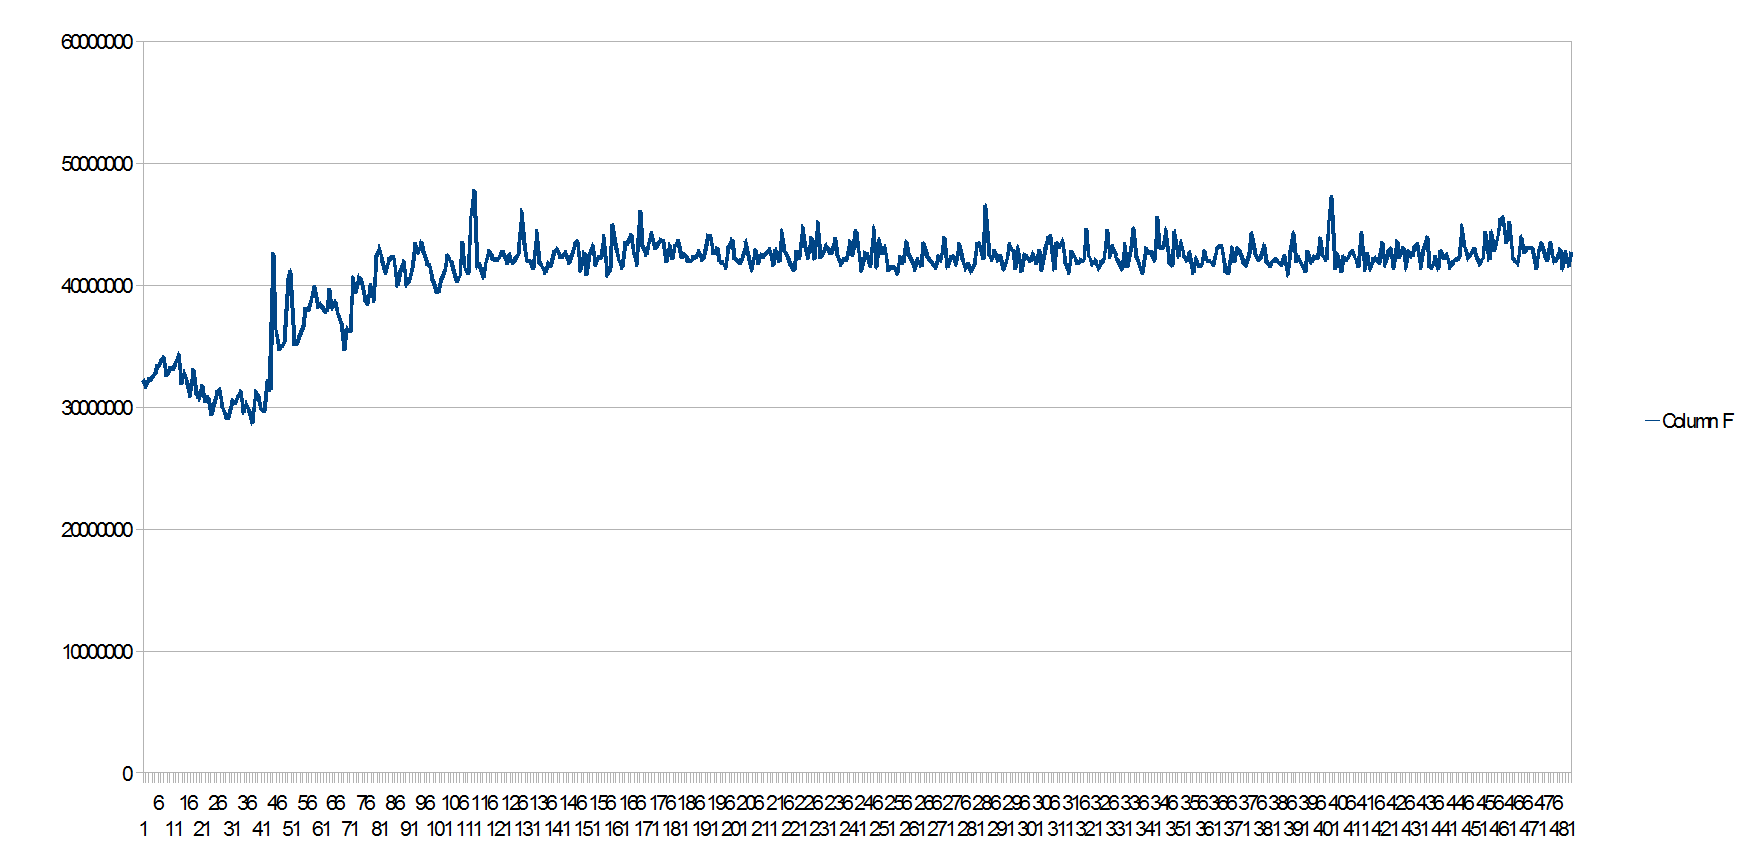
\includegraphics[width=1.00\textwidth]{Media/gpu_timer_hybrid.png}
	\caption{Output from GL TIME ELAPSED per frame for a hybrid scene. Time is averaging around 42.0 milliseconds.}	
	\label{fig:hybrid_gpu_time}
\end{figure}

\begin{figure}[H]
	\centering
	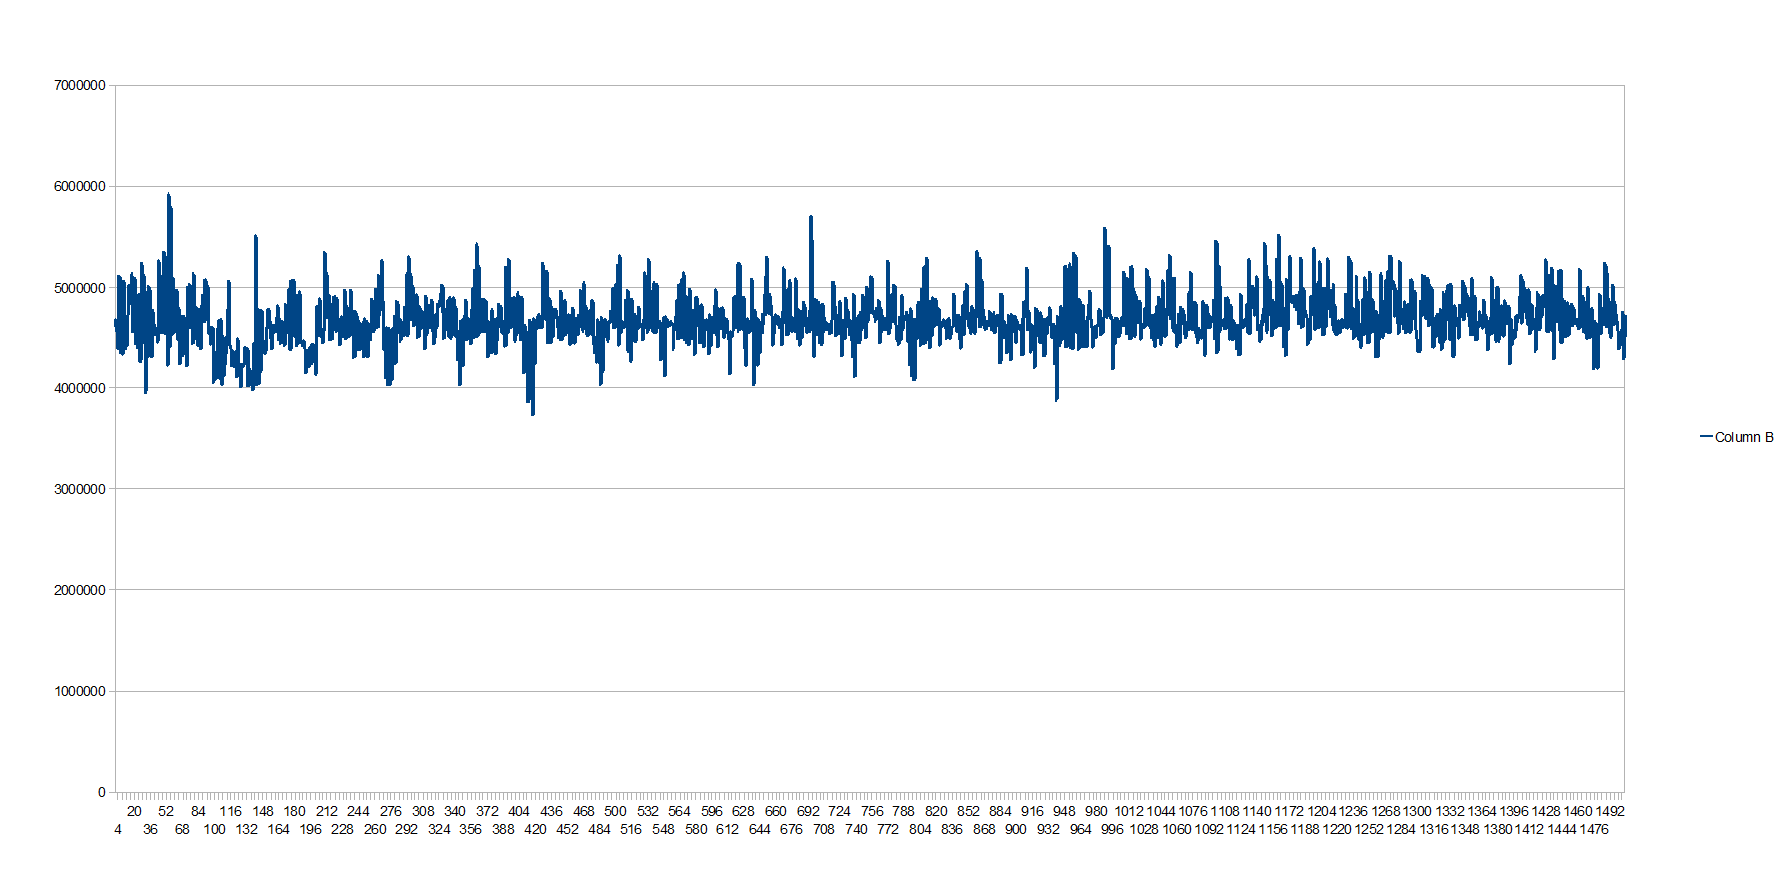
\includegraphics[width=1.00\textwidth]{Media/gpu_timer_raster_only.png}
	\caption{Output from GL TIME ELAPSED per frame for a purely rasterized scene. Time is averaging around 4.5 milliseconds.}
	\label{fig:raster_gpu_time}
\end{figure}

As figure \ref{fig:hybrid_gpu_time} and figure \ref{fig:raster_gpu_time} show, the hybrid scene is about ten times slower than the purely rasterized scene at a screen resolution of 1024x768.

\section{What went wrong}
In the end, the hybrid test configurations we managed to create were limited to raytracing the normals of the scene geometry and push that into the final deferred shading pass to use for lighting. We had a fully working raytraced shadows implementation in OptiX, but we couldn't get past some really bad crashes that was caused during interop, that just wouldn't allow us to move forward any further. Thus we never got to really test any hybrid configurations of true interest. But this was barely the icing on the cake of problems we encountered during the duration of our work.

The thesis was originally supposed to explore volume rendering with the OptiX raytracing framework, and how to combine that with a rasterized scene. We spent the good half of February 2012 researching volume rendering. We were thinking of exploring compositing volume graphics with typical solid-surface realtime graphics. Tile-based deferred rendering was of high interest to us, and we decided to study the ways this relatively new technique could be combined with realtime raytracing. Both deferred rendering with rasterization and raytracing are relatively old techniques that have recently become relevant for realtime graphics. Deferred pipelines became popular around 2004-2005 when GPUs finally had enough memory to allow multiple G-buffers to be held in memory. Raytracing on GPUs has become easy to program thanks to languages like OpenCL and CUDA. Since a deferred renderer outputs much of the information needed (surface position and normal) to start secondary rays, we thought combining the two could be advantageous.

We had an OpenGL based deferred renderer up and running fast, and the idea was to plug OptiX into this, as it seemingly had good interopability with OpenGL. Sadly, we spent a lot of time fighting crashes caused by OptiX and OpenGL interop. Having to wait for minutes to recover from display driver crashes sapped hours of development time, to the point where we were afraid this could damage our hardware. The retained-mode API-behaviour of OptiX hasn't helped when integrating it into our render-stage based framework either. OptiX isn't a bad library, it does what it claims very well, but it needs more users. For that to happen, it has to become more open and work on other vendors hardware. In hindsight, we should have written the raytracer ourselves.

Midway through the project, we decided we needed a scene that could showcase the properties of a hybrid. The BART project seemed like a perfect fit. One of the sample scenes contains mostly diffuse shaded geometry and some translucent geometry. It took some effort getting the BART parser into a workable state. The point of using BART was somewhat lost, as we didn't have time to implement the animation part of it, so, we couldn't compare our renderer against other implementations.

We didn't have a clear plan of distributing work between the rasterizer and the raytracer, this was supposed to be part of the experimentation of the thesis. Should only parts of the screen be raytraced? Should the raytracer handle soft omni-directional shadows? Should the rasterizer only handle its G-buffer creation, and OptiX the final shading? We tried to do too much. Much time was spent on details such as C++ design and architecture, and we greatly underestimated the effort it would take to get into the OptiX programming model.

\section{What went right}
We set out with a pretty solid engine architecture. Wrapping OpenGL functionality into object oriented code that would safely create and destruct itself, with simplified interfaces for interacting with the underlying OpenGL functionality worked really well.

